
\documentclass[runningheads]{llncs}

\usepackage[T1]{fontenc}
\usepackage{graphicx}

\begin{document}

\title{Modelado y Simulación de Producción de Alfajores Mediante SIMUL8}

\author{ZZZ Group}

\institute{Facultad de Ingeniería, Universidad Nacional de Cuyo}

\maketitle

\begin{resumen}
El presente trabajo describe el modelado y la simulación de una planta de producción de alfajores utilizando el software SIMUL8. El objetivo fue representar de manera detallada las distintas etapas del proceso productivo, desde la recepción de materias primas hasta el encajonado final del producto terminado. Para ello se configuraron diferentes centros de trabajo, colas, puntos de entrada y salida, incorporando distribuciones estadísticas, restricciones operativas, tiempos de espera y mecanismos de reutilización de material. La simulación permite analizar el comportamiento dinámico del sistema y evaluar su desempeño bajo condiciones representativas de operación industrial.

\keywords{SIMUL8 \and Simulación de eventos discretos \and Producción de alfajores \and Modelado de procesos}
\end{resumen}

\section{Introducción}

La simulación de eventos discretos constituye una herramienta ampliamente utilizada para el análisis y optimización de sistemas productivos. Mediante la representación de procesos, recursos y flujos de materiales, es posible estudiar el comportamiento de una planta industrial sin intervenir directamente sobre su operación real.

En el presente trabajo se desarrolló un modelo de simulación de una planta de producción de alfajores utilizando el software SIMUL8. El objetivo principal fue representar las diferentes etapas del proceso productivo, desde la recepción de materias primas hasta el encajonado del producto terminado, incorporando parámetros operativos, tiempos de procesamiento, controles de calidad y mecanismos de reutilización de material.

\section{Descripción del Modelo}
\begin{figure}
    \centering
    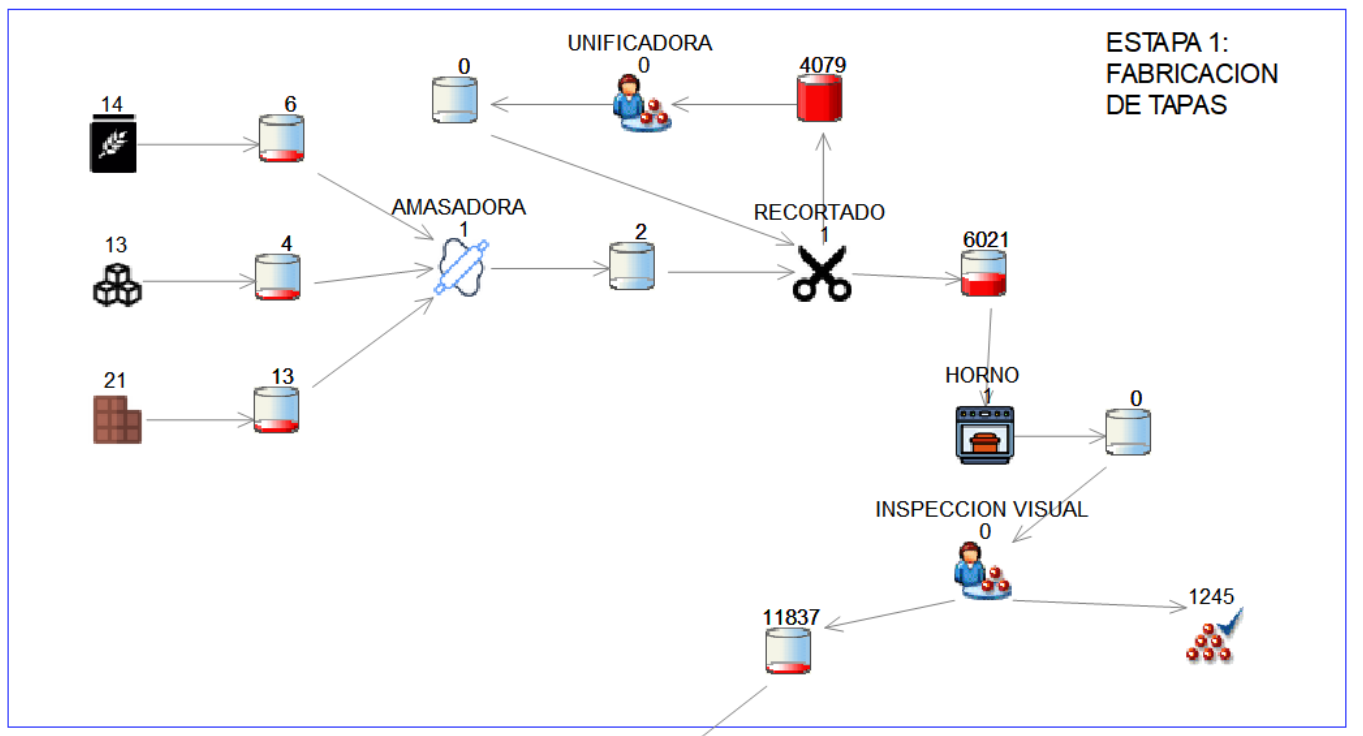
\includegraphics[width=0.75\linewidth]{Captura de pantalla 2026-06-03 023927.png}
    
    
\end{figure}
\begin{figure}
    \centering
    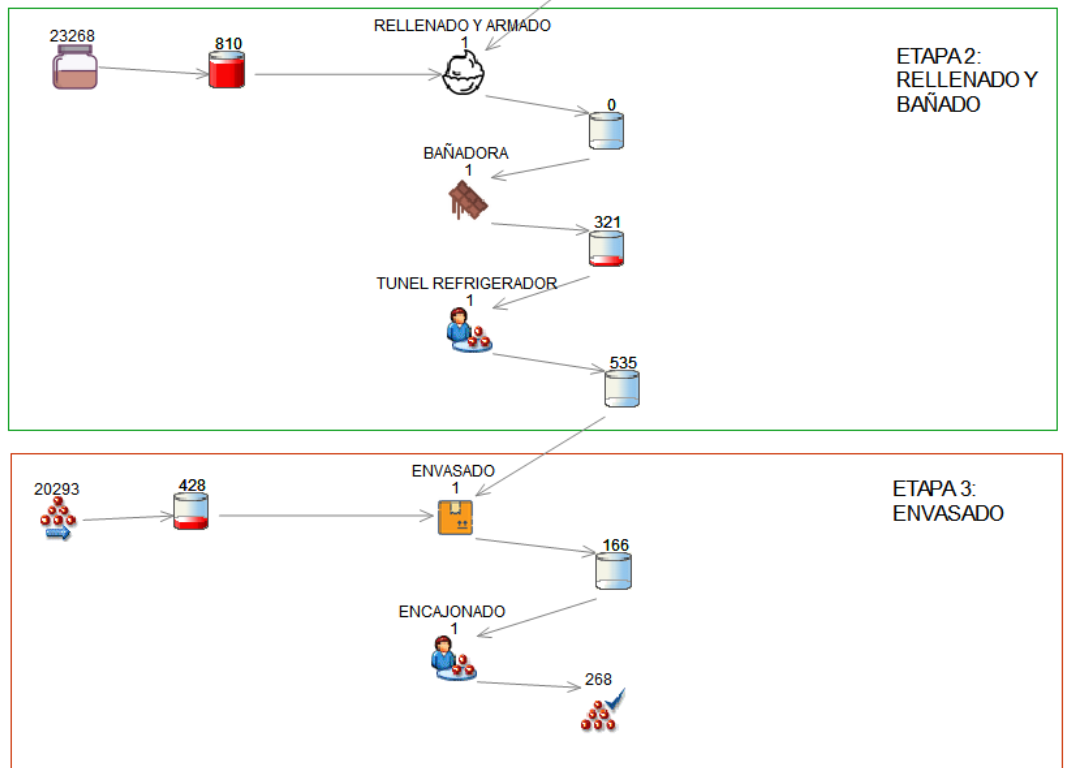
\includegraphics[width=0.75\linewidth]{Captura de pantalla 2026-06-03 024011.png}
    
    
\end{figure}
\subsection{Recepción de Materias Primas y Amasado}

La primera etapa del proceso corresponde a la recepción de harina, azúcar y cacao. Se decidió modelar cada insumo de manera independiente con el fin de representar con mayor precisión la disponibilidad de materias primas y generar colas específicas para cada ingrediente.

Cada punto de entrada fue configurado utilizando una distribución exponencial con un tiempo promedio de llegada de 40 minutos. Posteriormente, los tres insumos convergen en la amasadora, donde se implementó una distribución Average con un tiempo promedio de procesamiento de 40 minutos.

Debido a la modelación independiente de los ingredientes, el Routing In de la amasadora fue configurado para que el proceso se inicie únicamente cuando se encuentren disponibles simultáneamente una unidad de harina, una unidad de azúcar y una unidad de cacao. 

\subsection{Cámara de Frío}

Una vez completado el amasado, la masa es enviada a una cámara de frío donde permanece en reposo durante un período mínimo de 1 hora. Para representar esta operación se utilizó la función Min Wait Time con un valor de 60 minutos.

\subsection{Recortado y Reutilización de Material}

Luego del reposo, la masa ingresa al proceso de recortado.La duración del proceso fué definida en 45 minutos. La salida de este proceso fue configurada mediante la función Percent, estableciendo que el 75\% del material corresponde a galletas crudas aptas para continuar el proceso productivo, mientras que el 25\% restante corresponde a recortes sobrantes. Este proceso recibe como entrada un Item Type llamado LOTE MASA y entrega, mediante la función batching, 8000 unidades de otro Item llamado GALLETITA CRUDA.

Debido a restricciones asociadas al tipo de entidad manejado por SIMUL8, los recortes no pueden ser enviados directamente nuevamente al proceso. Por este motivo se incorporó una unificadora virtual encargada de acumular los recortes hasta alcanzar un total de 8000 unidades. Una vez alcanzada dicha cantidad, los recortes son transformados nuevamente en un lote de masa y reingresan a la línea de producción.

Además, se otorgó prioridad a los recortes de masa permitiendo su reincorporación preferencial al sistema.

\subsection{Horneado}

Las galletas crudas obtenidas del recortado son enviadas al horno. El proceso de horneado fue modelado mediante una distribución Average con un tiempo promedio de 5 minutos.

El Routing In utiliza la función Collect, estableciendo la necesidad de reunir 800 galletas crudas antes de iniciar el ciclo de horneado. El Routing Out fue configurado para liberar exactamente 800 unidades, manteniendo la conservación de la producción procesada. Durante esta etapa se produce además el cambio de tipo de entidad desde galleta cruda hacia galleta cocida.

\subsection{Inspección Visual y Secado}

Después del horneado, las galletas cocidas atraviesan una etapa de inspección visual. La salida del proceso se configuró mediante la función Percent, asignando una probabilidad del 98\% a unidades aptas y del 2\% a unidades defectuosas. A este proceso se le asigno un tiempo igual a cero ya que no interrumpe el circulamiento del producto. 

Las unidades rechazadas son enviadas a un End Point. Las unidades aprobadas continúan hacia una cola denominada Tapitas en Descanso, donde permanecen durante 1 hora para eliminar la humedad residual. Este comportamiento fue modelado mediante la función Min Wait Time con un valor de 60 minutos.

\subsection{Rellenado y Armado}

La segunda fase del proceso incorpora un nuevo punto de entrada correspondiente al dulce de leche. En el centro de trabajo denominado Rellenado y Armado se combinan dos tapitas secas con una dosis de dulce de leche para conformar un alfajor.

Esta operación fue configurada mediante la función Collect en el Routing In. La velocidad de procesamiento fue definida en 0,0125 minutos por unidad, equivalente a una capacidad de producción de 80 alfajores por minuto.

\subsection{Bañado}

Una vez armados, los alfajores ingresan al proceso de bañado con chocolate. Esta etapa fue configurada utilizando la misma distribución y velocidad de procesamiento empleadas durante el rellenado. Para este proceso se supuso una recirculación de chocolate continua por motivos de simplificación del modelo.

\subsection{Túnel de Refrigeración}

Posteriormente, los alfajores bañados son enviados a un túnel de refrigeración donde el chocolate se endurece y adquiere las condiciones adecuadas para la comercialización. 

El túnel fue modelado mediante una distribución Average con un tiempo de procesamiento de 7 minutos. Asimismo, se configuró la función Collect para reunir un lote de 560 alfajores antes de iniciar el proceso y una salida igual.

\subsection{Envasado}

En la última etapa de producción se realiza el envasado individual de los alfajores. El proceso fue configurado utilizando una distribución Fixed y una velocidad de producción equivalente a 80 alfajores por minuto (0,0125).

El Routing In se programó para unir una unidad de producto con una unidad de envase, con la función Collect y Assemble,  generando como resultado un alfajor envasado.

\subsection{Encajonado}

Finalmente, los alfajores envasados son agrupados en cajas para su almacenamiento y distribución. La operación se modeló mediante la función Collect, estableciendo la necesidad de reunir 80 alfajores por caja.

El tiempo de procesamiento fue definido mediante una distribución Average con un valor promedio de 1 minuto.

\section{Configuración del Reloj de Simulación}

Con el fin de evitar que las condiciones iniciales afecten los resultados obtenidos, se implementó la función Warm Up Period. Esta configuración permite descartar una porción inicial de la simulación, correspondiente a la puesta en marcha del sistema y al llenado progresivo de las distintas etapas productivas.

Para ello se tomó un tiempo de calentamiento de 180 min (3 hs).De esta manera, los indicadores analizados reflejan el comportamiento estable de la planta, proporcionando resultados más representativos y confiables. 

Por último se utilizó la función Simple unit count from zero para poder generalizar los resultados del proceso a cualquier periodo. Y se configuró el Result collection period en 480 minutos (8 hs), simulando así un turno de trabajo en la planta. 

\section{Resumen de Configuraciones del Modelo}

\subsection{Nota de Simplificación y Supuestos de Modelado}

Para optimizar el rendimiento computacional del software y agilizar los tiempos de procesamiento, se aplicó una simplificación analítica sobre los tiempos de espera pasivos. Los períodos de estacionamiento en la \textbf{Cámara de Frío} (reposo de la masa) y en el \textbf{Almacén de Descanso de Tapas} (enfriamiento post-horno), cuyos valores reales son de 24 horas respectivamente, se parametrizaron en \textbf{60 minutos} dentro del modelo.

\textit{Sustento técnico:} Al tratarse de operaciones de almacenamiento estático que no generan cuellos de botella dinámicos por falta de personal o maquinaria activa, esta reducción no altera la capacidad máxima de producción de la línea ni el comportamiento de los procesos clave (Amasado, Cortado, Rellenado y Empaque). Esto permite analizar el \textbf{Estado Estable (Steady State)} de la planta en un horizonte de tiempo simulado más eficiente sin alterar la validez del balance de masa.

 
Con el objetivo de facilitar la interpretación del modelo desarrollado, la Tabla 1 resume las principales configuraciones implementadas en cada etapa de la línea de producción.

\begin{figure}
    \centering
    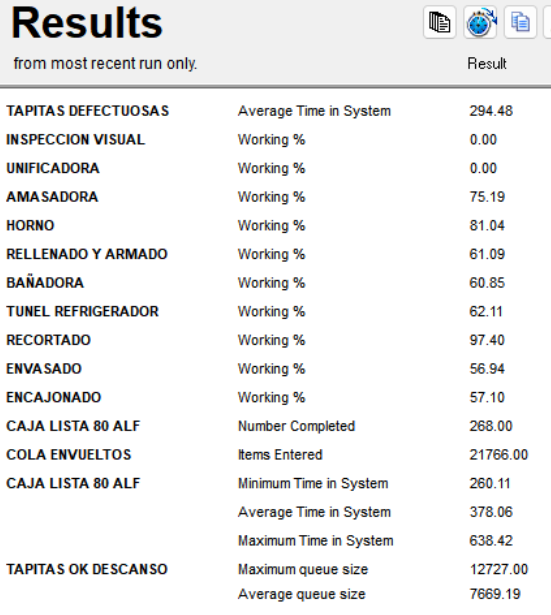
\includegraphics[width=1\linewidth]{TABLA 1.png}
    \caption{Enter Caption}
    \label{fig:placeholder}
\end{figure}
\section{Resultados de la Simulación}

Con el fin de evaluar el desempeño de la planta modelada, se realizaron 5 corridas de simulación utilizando los parámetros previamente definidos. Los resultados obtenidos permitieron analizar el comportamiento de la línea de producción, la utilización de los recursos y el impacto de las restricciones impuestas por los procesos que operan por lotes.

La Tabla 1 resume los principales indicadores de desempeño obtenidos a partir de las corridas realizadas.

\subsection{Interpretación de los Indicadores de Rendimiento (KPIs)}

\begin{itemize}
    \item \textbf{Identificación del Cuello de Botella Absoluto:} La actividad \textbf{RECORTADO} presenta un porcentaje de ocupación crítico del \textbf{97.40\%}. Esto demuestra que es la operación restrictiva de la planta. La velocidad general de toda la fábrica de alfajores está dictada por la capacidad de troquelado de esta máquina. Cualquier proyecto de inversión o mejora de métodos destinada a aumentar el \textit{throughput} global de la empresa debe enfocarse obligatoriamente en este nodo.
    \item \textbf{Eficiencia de la Cocción y Preparación:} El \textbf{HORNO} opera a un \textbf{81.04\%} de su capacidad, lo que indica un nivel de utilización alto y saludable, encontrándose correctamente sincronizado (un paso por detrás) con la velocidad del Recortado. Por su parte, la \textbf{AMASADORA (75.19\%)} demuestra un funcionamiento eficiente gracias a las restricciones de capacidad máxima (\textit{Max Capacity}) implementadas en las colas intermedias, logrando autorregularse y evitar la sobreproducción de masa.
    \item \textbf{Sincronización del Bloque de Armado y Cobertura:} Las actividades de \textbf{RELLENADO Y ARMADO (61.09\%)}, \textbf{BAÑADORA (60.85\%)} y \textbf{TÚNEL REFRIGERADOR (62.11\%)} muestran porcentajes de utilización prácticamente idénticos. Esto evidencia un \textbf{flujo continuo y balanceado} en la segunda mitad de la línea. Este bloque cuenta con un margen de capacidad ociosa (aprox. 38\%) que le permitiría absorber incrementos de producción si en el futuro se optimiza el sector de cortado.
    \item \textbf{Rendimiento Logístico y Output:} El proceso de empaque (\textbf{ENVASADO: 56.94\%} y \textbf{ENCAJONADO: 57.10\%}) acompaña fluidamente el ritmo de la planta, logrando un output total de \textbf{268 cajas listas de 80 alfajores} (21,440 unidades finalizadas en caja) para el período bajo análisis, con un tiempo promedio de permanencia en el bloque de empaque secundario de \textbf{378.06 minutos} por lote de cajas.
    \item \textbf{Promedio de la cola en el secado (7.669 tapitas): El Pulmón del Proceso} Representa el stock normal que vive en la zona de descanso. Demuestra que la cola cumple su función de \textbf{"colchón de seguridad"}, garantizando que al sector de Rellenado nunca le falte materia prima, permitiéndole trabajar de forma fluida y continua.
    \item \textbf{Máximo de la cola en el secado (12.727 tapitas): El Límite de Diseño Físico} Es el dato más importante para la infraestructura. Determina el \textbf{tamaño real que debe tener el área de almacenamiento} en la planta. La fábrica debe diseñarse con espacio, carros y estanterías suficientes para soportar este pico de 12.727 tapitas en simultáneo, evitando que el stock desborde el sector y termine trabando el Horno hacia atrás. 
    \item \textit{(Nota: Las actividades con 0.00\% de uso corresponden a bloques de lógica instantánea parametrizados con tiempo de operación cero, por lo que no consumen minutos del reloj de simulación)}.
\end{itemize}
 

\section{Posibles Mejoras del Sistema}

A partir del comportamiento observado durante las corridas de simulación, se identificaron diversas oportunidades de mejora que podrían incrementar la productividad de la planta.

Entre las alternativas más relevantes se destacan:

\begin{itemize}

\subsubsection{1. Optimizar el Recortado (Atacar el Cuello de Botella)}

Como la cortadora trabaja al \textbf{97.40\%}, es el límite de la planta. Proponer una cuchilla múltiple o mayor velocidad para reducir su tiempo de ciclo aumentará automáticamente la producción total de alfajores.

\subsubsection{2. Controlar el tamaño del secado}

Colocar sensores en la cola de descanso de tapas. Cuando llegue a un límite seguro (ej. 8,000 unidades), que envíe una señal para frenar temporalmente la Amasadora. Esto evitará el pico de \textbf{12,727 tapitas} y achicará el tamaño necesario de la habitación.

\subsubsection{3. Sincronizar el Bloque de Terminación (Flujo Continuo)}

Unificar mecánicamente las estaciones de Rellenado, Bañado y Túnel de frío en una sola línea integrada con velocidad regulable, aprovechando que las tres trabajan sintonizadas en torno al \textbf{61\%}.

\subsubsection{4. Automatizar el Encajonado (Agilizar la Logística)}

Implementar un sistema de empaque automático para armar las cajas de 80 alfajores más rápido, reduciendo el tiempo promedio de permanencia de la caja terminada (\textbf{378 minutos}) en el sector de despacho.

 
\end{itemize}

Estas alternativas podrían evaluarse mediante futuras corridas de simulación, permitiendo cuantificar sus beneficios antes de implementar modificaciones reales en la planta.

\section{Conclusiones}

El modelo desarrollado permitió representar de forma detallada el funcionamiento de una planta de producción de alfajores, incorporando aspectos relevantes como la sincronización de insumos, el trabajo por lotes, la reutilización de material, los controles de calidad y los tiempos de reposo requeridos por el proceso.

La utilización de SIMUL8 facilitó la construcción de un entorno capaz de reproducir las condiciones operativas de una línea de producción real, permitiendo analizar cuellos de botella, niveles de utilización y comportamiento general del sistema.

\begin{thebibliography}{2}

\bibitem{simul8}
SIMUL8 Corporation: SIMUL8 User Manual and Documentation.

\bibitem{alfajores}
Información técnica y referencias de procesos productivos observados en plantas industriales de elaboración de alfajores.

\end{thebibliography}

\end{document}
